% Original book diagram: fig:dt_assimilation
% Book source: sections/Part_V/DT.tex
% Original diagram authorship retained. Visual design: Ziad Mosalam.
\documentclass[11pt,border=8pt]{standalone}
\usepackage{amsmath,amssymb,graphicx,tikz}
\usetikzlibrary{arrows.meta,automata,positioning,calc,shapes.geometric,fit,backgrounds,patterns}
\newcommand{\vect}[1]{\mathbf{#1}}
\newcommand{\mat}[1]{\mathbf{#1}}
\newcommand{\Normal}{\mathcal{N}}
\newcommand{\prob}{p}
\newcommand{\E}{\mathbb{E}}
\newcommand{\Var}{\mathrm{Var}}
\newcommand{\Cov}{\mathrm{Cov}}
\newcommand{\CovP}{\mathbf{P}}
\newcommand{\Prob}{\mathbb{P}}
\setlength{\textwidth}{6.5in}
% Shared visual vocabulary for the book's original diagrams.
% Figures opt in explicitly, so unrelated text and existing additions are unchanged.
\definecolor{BookBlue}{HTML}{003262}
\definecolor{BookGold}{HTML}{B17A00}
\definecolor{BookTeal}{HTML}{247C86}
\definecolor{BookInk}{HTML}{30363B}
\definecolor{BookLight}{HTML}{E9EFF5}
\tikzset{
  book figure/.style={font=\small\rmfamily, color=BookBlue, text=BookInk,
    line width=0.8pt, >=Latex},
  book axis/.style={->, draw=BookInk, line width=0.6pt},
  book link/.style={->, draw=BookBlue, line width=0.8pt},
  book observation/.style={draw=BookGold, fill=BookGold!8},
  book state/.style={draw=BookBlue, fill=BookLight},
  book note/.style={font=\footnotesize\rmfamily, text=BookInk}
}

\begin{document}
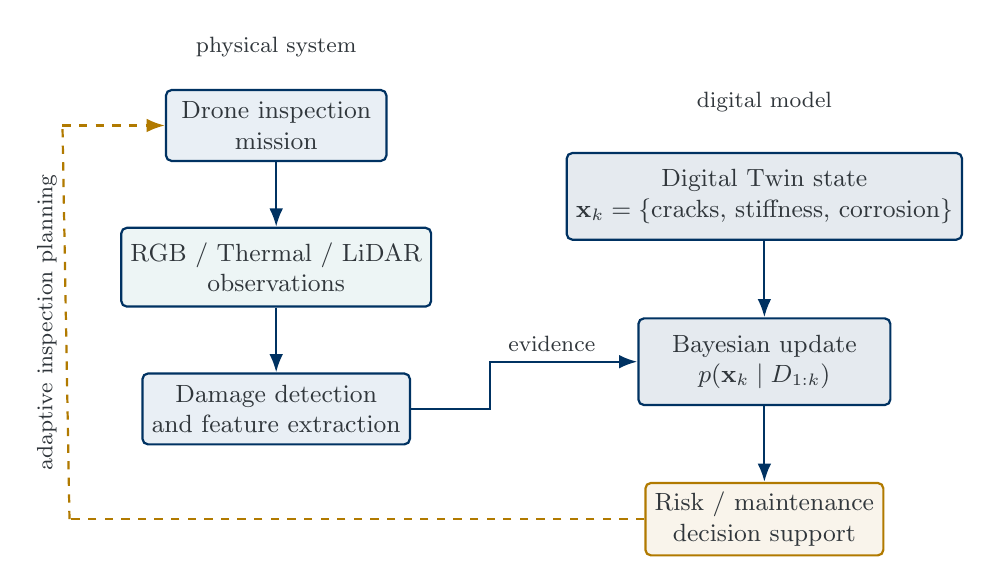
\begin{tikzpicture}[book figure,
    >=Latex,
    every node/.style={font=\small, align=center},
    block/.style={
        rectangle,
        rounded corners=2pt,
        draw,
        minimum width=2.8cm,
        minimum height=0.9cm,
        line width=0.8pt,
        fill=BookLight
    },
    stateblock/.style={
        rectangle,
        rounded corners=2pt,
        draw,
        minimum width=3.2cm,
        minimum height=1.1cm,
        line width=0.8pt,
        fill=BookBlue!10
    },
    obsblock/.style={
        rectangle,
        rounded corners=2pt,
        draw,
        minimum width=3.0cm,
        minimum height=1.0cm,
        line width=0.8pt,
        fill=BookTeal!8
    },
    arrow/.style={->, draw=BookBlue, line width=0.8pt}
]

% Left column: physical / sensing
\node[block] (drone) at (0,2.2) {Drone inspection\\mission};
\node[obsblock] (obs) at (0,0.4) {RGB / Thermal / LiDAR\\observations};
\node[block] (vision) at (0,-1.4) {Damage detection\\and feature extraction};

% Right column: twin / state
\node[stateblock] (state) at (6.2,1.3) {Digital Twin state\\$\vect{x}_k = \{\text{cracks, stiffness, corrosion}\}$};
\node[stateblock] (update) at (6.2,-0.8) {Bayesian update\\$\prob(\vect{x}_k \mid D_{1:k})$};
\node[block,draw=BookGold,fill=BookGold!8] (risk) at (6.2,-2.8) {Risk / maintenance\\decision support};

% Arrows in left column
\draw[arrow] (drone) -- (obs);
\draw[arrow] (obs) -- (vision);

% Orthogonal arrow from vision to update
\draw[arrow] (vision.east) -- ++(1.0,0)
             |- node[pos=0.55, above, xshift = 0.6cm] {\footnotesize evidence} (update.west);

% Arrows in right column
\draw[arrow] (state) -- (update);
\draw[arrow] (update) -- (risk);

% Feedback loop: horizontal out, vertical up, horizontal in
\draw[dashed, draw=BookGold, line width=0.8pt]
(risk.west) -- ([xshift=-7.3cm]risk.west);

\draw[dashed, draw=BookGold, line width=0.8pt]
([xshift=-7.3cm]risk.west) -- ([xshift=-1.3cm]drone.west);

\draw[arrow, draw=BookGold, dashed, line width=0.8pt]
([xshift=-1.3cm]drone.west) -- (drone.west);

% Rotated label centered on vertical segment
\node[rotate=90, font=\footnotesize]
at ([xshift=-1.5cm,yshift=-2.5cm]drone.west) {adaptive inspection planning};

% Column notes
\node[font=\footnotesize] at (0,3.2) {physical system};
\node[font=\footnotesize] at (6.2,2.5) {digital model};

\end{tikzpicture}
\end{document}
